%%%%%%%%%%%%%%%%%%%%%%%%%%%%%%%%%%%%%%%%%
% fphw Assignment
% LaTeX Template
% Version 1.0 (27/04/2019)
%
% This template originates from:
% https://www.LaTeXTemplates.com
%
% Authors:
% Class by Felipe Portales-Oliva (f.portales.oliva@gmail.com) with template 
% content and modifications by Vel (vel@LaTeXTemplates.com)
%
% Template (this file) License:
% CC BY-NC-SA 3.0 (http://creativecommons.org/licenses/by-nc-sa/3.0/)
%
%%%%%%%%%%%%%%%%%%%%%%%%%%%%%%%%%%%%%%%%%

%----------------------------------------------------------------------------------------
%    PACKAGES AND OTHER DOCUMENT CONFIGURATIONS
%----------------------------------------------------------------------------------------

\documentclass[
    12pt, % Default font size, values between 10pt-12pt are allowed
    %letterpaper, % Uncomment for US letter paper size
    %spanish, % Uncomment for Spanish
]{fphw}

% Template-specific packages
\usepackage[utf8]{inputenc} % Required for inputting international characters
\usepackage[T1]{fontenc} % Output font encoding for international characters
\usepackage{fontspec,unicode-math} % Required for using utf8 characters in math mode
\usepackage{parskip}  % To add extra space between paragraphs
% \usepackage{mathpazo} % Use the Palatino font
\usepackage{graphicx} % Required for including images
\usepackage{booktabs} % Better horizontal rules in tables
\usepackage{hyperref} % For links (both internal and external)
% \usepackage{listings} % Required for insertion of code
\usepackage{enumerate}% To modify the enumerate environment
\usepackage{cleveref} % Better \ref command -> \cref
\usepackage{import}   % This 4 packages and the command allow importing pdf
\usepackage{xifthen}  % figures generated with inkscape
\usepackage{pdfpages} % Source: https://castel.dev/post/lecture-notes-2/
\usepackage{mathtools}
\usepackage{wrapfig}
\usepackage{cancel}
\usepackage{transparent}
\newcommand{\incfig}[1]{%
    \def\svgwidth{0.95\columnwidth}
    \small
        \import{./images/}{#1.pdf_tex}
}

\setlength{\parindent}{15pt}
\setlength{\headheight}{22.66pt}

%----------------------------------------------------------------------------------------
%    ASSIGNMENT INFORMATION
%----------------------------------------------------------------------------------------

\title{Task 4 \\ Hyperbolic paraboloid} % Assignment title

\author{Emilio Domínguez Sánchez} % Student name

\date{October 28th, 2020} % Due date

\institute{University of Murcia \\ Faculty of Mathematics} % Institute or school name

\class{Geometría de Superficies} % Course or class name

\professor{Dr. Pascual Lucas Saorin} % Professor or teacher in charge of the assignment

%----------------------------------------------------------------------------------------
%    Definitions
%----------------------------------------------------------------------------------------

\makeatletter
\newcommand{\defined}[2]{%
  \phantomsection
  \textit{#1}\def\@currentlabel{\unexpanded{#1}}\label{#2}%
}
\makeatother

\usepackage{physics}
\DeclareMathOperator{\Ima}{Im}
\DeclareMathOperator{\sgn}{sgn}
\DeclareMathOperator{\arctanh}{arctanh}
\newcommand{\R}{\mathbb{R}}
\newcommand{\Z}{\mathbb{Z}}

\begin{document}

\maketitle % Output the assignment title, created automatically using the information in the custom commands above

%----------------------------------------------------------------------------------------
%    ASSIGNMENT CONTENT
%----------------------------------------------------------------------------------------

\section*{Problem}

\begin{problem}

Prove that the set

\begin{equation*}
    S = \qty{\mqty(x & y & z) \in \R^3 : z = x^2 - y^2}
\end{equation*}

is a regular surface.
Show that the following maps are parametrizations of $S$.

\begin{align*}
    X\mqty(u & v) &= \mqty(u+v & u-v & 4uv), & \mqty(u & v) \in \R^2 \\
%
    Y\mqty(u & v) &= \mqty(u\cosh v & u\sinh v & u^2), & u \neq 0, \mqty(u & v) \in \R^2
\end{align*}

Which parts of $S$ are covered by this parametrizations?

\end{problem}

%----------------------------------------------------------------------------------------

\subsection*{Answer}

    From its definition it is clear that $S$ is the graph of the differentiable function
$z\mqty(x & y) = x^2 - y^2$.
We already know that this is a sufficient condition to be a regular surface.
It will be useful to call $\mqty(x & y) \mapsto \mqty(x & y & z\mqty(x & y))$ the
\defined{standard parametrization}{name:std-par}.

\subsubsection*{Map $X$}

    We will first show that $X$ is a parametrization of all $S$.
Notice that $\mqty(u & v) \mapsto \mqty(u+v & u-v)$ is a change of coordinates in $\R^2$.
You can either realize that $\mqty(1 & 1)$ and $\mqty(1 & -1)$ are independent vectors,
that is,
that it is a linear map of maximum range;
or prove that it has inverse solving a system of equations.

\begin{align*}
    \begin{cases}
        x = u + v \\
        y = u - v \\
    \end{cases}
    \iff
    \begin{cases}
        u = \frac{x+y}{2} \\
        v = \frac{x-y}{2} \\
    \end{cases}.
\end{align*}

\noindent
Hence, $X$ can be written as the composition (\cref{eq:x-is-comp})
of the \ref{name:std-par} with the change of coordinates,
which shows that the image of $X$ is the same as the image of the
standard parametrization,
the whole $S$.

\begin{equation}\label{eq:x-is-comp}
    \begin{aligned}
        X\mqty(u & v) =& \quad
        \mqty(u+v & u-v & 4uv) = \\
        & \quad
        \mqty(u+v & u-v & (u+v)^2-(u-v)^2) = \\
        & \quad
        \mqty(u+v & u-v & z\mqty(u+v & u-v)), \\
%
        X =& \quad
        \qty[\mqty(x & y) \mapsto \mqty(x & y & z\mqty(x & y))]
        \quad \circ \quad
        \qty[\mqty(u & v) \mapsto \mqty(u+v & u-v)].
    \end{aligned}
\end{equation}

    This shows that $X$ is
differentiable because it's the composition of two differentiable maps,
an homeomorphism because it is the composition of two homeomorphisms and
has a maximum range differential $\dd X_p$ for all $p$,
because the differential is the composition of the differentials of those functions,
both of maximum range.
Thus, $X$ is a parametrization.

\subsubsection*{Map $Y$}

    It is easier to work with the second map if we are familiarized with
the concepts of hyperbola and hyperbolic functions.
First, $\Ima Y \subset S$ because $\cosh^2 t - \sinh^2 t = 1$.
But we will see that in this case the parametrization does not cover $S$.
As before, we can write $Y$ as the composition

\begin{equation*}
    Y =
    \qty[\mqty(x & y) \mapsto \mqty(x & y & z\mqty(x & y))]
    \quad \circ \quad
    \qty[\mqty(u & v) \mapsto \mqty(u\cosh v & u\sinh v)].
\end{equation*}

\noindent
Call the restricted map
$\mqty(u & v) \mapsto \mqty(u\cosh v & u\sinh v) \eqqcolon y$.
The decomposition means, as before,
that $Y$ will be a parametrization if $y$ is it.
And, also, that we can study the points in the image of $Y$ by
studying the points of $\R^2$ in the image of $y$ and then proyecting them onto $S$.

\begin{wrapfigure}[15]{l}{0.4\textwidth}
    \centering
    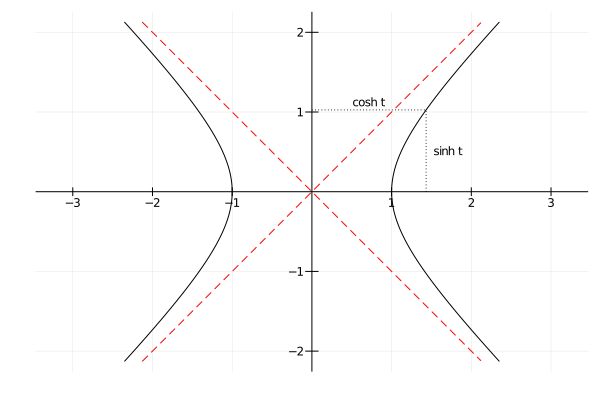
\includegraphics[width=0.36\textwidth]{images/hyperbola.png}
    \caption{How the right blade of the hyperbola $1 = x^2-y^2$ is parametrized.}
    \label{fig:hyperbola}
\end{wrapfigure}

    Write $\mqty(u\cosh v & u\sinh v) = u\mqty(\cosh v & \sinh v)$.
We see that the purpose of $u$ is to scale the curve
$\qty{\mqty(\cosh t, \sinh t)}_{t \in \R}$
through $\R^2$.
(Note that this curve is a hyperbola (\cref{fig:hyperbola}),
as would the curve with standard trigonometric functions be a circle.)

    Hence, the points are those either in the hyperbola $1 = x^2-y^2$,
of the form $\mqty(\cosh v & \sinh v)$,
or in the line that passes through the origin and such a point,
exceptuating the origin itself because $u \neq 0$.

    If we know about the hyperbola and that it approximates to the asymptotes
$x = y$ and $x = -y$,
we can already guess graphically that the image of our map is
the part enclosed by the red lines in \cref{fig:hyperbola},
precisely the two quarters of the plane where the hyperbola is drawn:

\begin{equation}\label{eq:imy}
    \Ima y = \qty{ρ\mqty(1 & c) : ρ \neq 0, ρ \in \R, c \in (-1, 1)}.
\end{equation}

    How can we prove the whole exercise formally and with the least possible hassle?

\subsection*{Differentiability}

    $y$ is easily differentiable.

\begin{align*}
    \pdv{y}{u} = \pdv{u} \mqty(u\cosh v & u\sinh v) =& \mqty(\cosh v & \sinh v), \\
    \pdv{y}{v} = \pdv{v} \mqty(u\cosh v & u\sinh v) =& u\mqty(\sinh v & \cosh v).
\end{align*}

\subsection*{Maximal range differential}

    Find the determinant of the differential.

\begin{equation*}
    \mdet{\mqty{\pdv{y}{u} & \pdv{y}{v}}} =
    \mdet{\mqty{\cosh v & u\sinh v \\ \sinh v & u\cosh v}} =
    u\cosh^2 v - u\sinh^2 v =
    u \neq 0.
\end{equation*}

\subsection*{Homeomorphism} Find inverse and see that it is continuous.

Working on the system of equations

\begin{equation*}
    \begin{cases}
        x = u\cosh v \\
        y = u\sinh v
    \end{cases},
\end{equation*}

\noindent
we get that $u^2 = x^2-y^2$ and that $\tanh{v} = \frac{y}{x}$.
Because $\cosh v > 0$, $\sgn{x} = \sgn{u}$ and we get

\begin{equation*}
    \begin{cases}
        u = \qty(\sgn{x}) \sqrt{x^2-y^2} \\
        v = \arctanh{\frac{y}{x}}
    \end{cases}.
\end{equation*}

\noindent
And to prove the previous expression
is an inverse we compose both functions\footnotemark.

\footnotetext{Two elementary results.
An surjective function (therefore any function restricted to its image)
has a right inverse.
The problem is always finding a left inverse,
equivalently seeing that the function is inyective,
which we check we have done by compositing the functions in the proper order.
And if a function is both injective and surjective,
any left (resp. right) inverse is also a right (resp. left) inverse.
As a conclusion, it is not necessary to compose the functions the other way around.}

\begin{equation*}
    \begin{cases}
        \sgn{(u\cosh v)} \sqrt{u^2\cosh v - u^2\sinh v} =
        \sgn u\abs{u} =
        u \\
        \arctanh{\frac{u\sinh v}{u\cosh v}} =
        \arctanh{\tanh v} =
        v
    \end{cases}.
\end{equation*}

\noindent
The inverse is continuous because each coordinate is made by
composing and performing elementary operations over continuous functions.
The only exception would be the functions $\sgn(x)$ and $\frac{y}{x}$,
which are discontinuous when $x = 0$.
But the inverse is not defined on $x = 0$ because $x = u\cosh v$,
$u \neq 0$, $\cosh v > 0$.

\subsection*{Image in $\R^2$}

    Use the formulas for the hyperbolic sine and cosine.

\begin{equation*}
    \cosh v = e^v - e^{-v} \qquad \sinh v = e^v + e^{-v}
\end{equation*}

    Therefore, for any point $\mqty(x & y) = u\mqty(\cosh v, \sinh v)$,
and the coefficient

\begin{equation*}
    c = \frac{y}{x} = \frac{e^v-e^{-v}}{e^v+e^{-v}} = 1 - 2\frac{e^{-v}}{e^v+e^{-v}}.
\end{equation*}

\noindent
$0 < \frac{e^{-v}}{e^v+e^{-v}} < 1$ because the exponential is always positive.
But the fraction takes the values over the whole interval $(0, 1)$ because

\begin{equation*}
    \lim_{v \to \infty}
        \frac{\cancelto{0}{e^{-v}}}{\cancelto{\infty}{e^v + e^{-v}}} \quad = 0
    \qquad
    \lim_{v \to -\infty}
        \frac{e^{-v}}{\cancelto{0}{e^v} + e^{-v}} = 1.
\end{equation*}

\noindent
This proves that the values of $c$ along all the hyperbola are the interval $(-1, 1)$,
which means that the \cref{eq:imy} was a correct guess.

\subsection*{Conclusions for the map Y}

    We proved that the map $y$ was differentiable with a differential of maximum range
and an homeomorphism.
Thus, so is $Y$.

To conclude the exercise, we give an expression for the image of $Y$
knowing the image of $y$.

\begin{multline*}
    \Ima Y = \\
    \qty[\mqty(x & y) \mapsto \mqty(x & y & z\mqty(x & y))] (\Ima y) = \\
    y (\qty{ρ\mqty(1 & c) : ρ \neq 0, ρ \in \R, c \in (-1, 1)}) = \\
    \qty{\mqty(ρ & ρc & ρ^2(1-c^2)) : ρ \neq 0, ρ \in \R, c \in (-1, 1)}).
\end{multline*}

Note that $\Ima y$ is the set of points of the plane where $\abs{y} < \abs{x}$
and $\Ima Y$ is the part of $S$ where $z$ is strictly positive.

\section*{Extra: Images}

    I present in this section two graphics of $S$.
I created this graphics and the \cref{fig:hyperbola} using
\href{https://julialang.org/}{Julia}.

\begin{figure}[h]
    \begin{minipage}{0.5\textwidth}
        \centering
        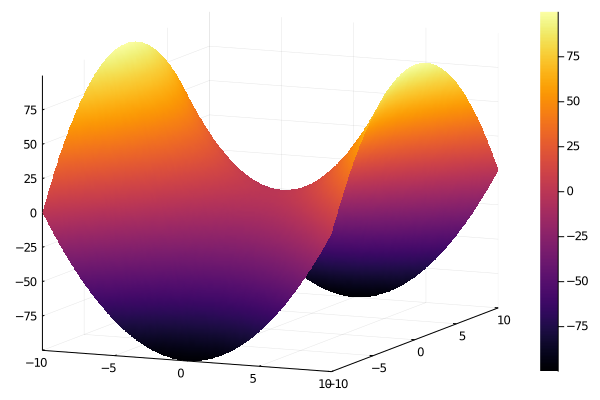
\includegraphics[width=\textwidth]{images/hyperbolic-paraboloid.png}
        \caption{The surface $S$. \\ A hyperbolic paraboloid.}
    \end{minipage}%
%
    \begin{minipage}{0.5\textwidth}
        \centering
        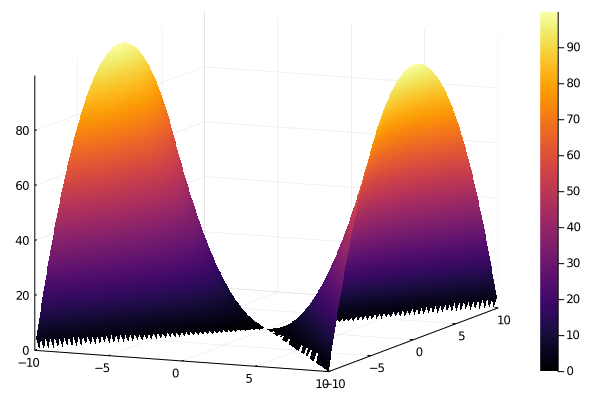
\includegraphics[width=\textwidth]{images/image-parametrization-Y.png}
        \caption{$\Ima Y$.}
    \end{minipage}
\end{figure}

%----------------------------------------------------------------------------------------

\end{document}
